\sloppy
\section{Python Basic Operator}


\vspace{12pt}
\noindent 
Operator adalah konstruksi yang dapat memanipulasi nilai operan. \par
\vspace{12pt}
\noindent 
Perhatikan ungkapan 4 + 5 = 9. Di sini, 4 dan 5 disebut operan dan + disebut operator. \par
\vspace{12pt}
\noindent 

\subsection{Jenis Operator}
 
\begin{figure}[ht]
 	\centerline{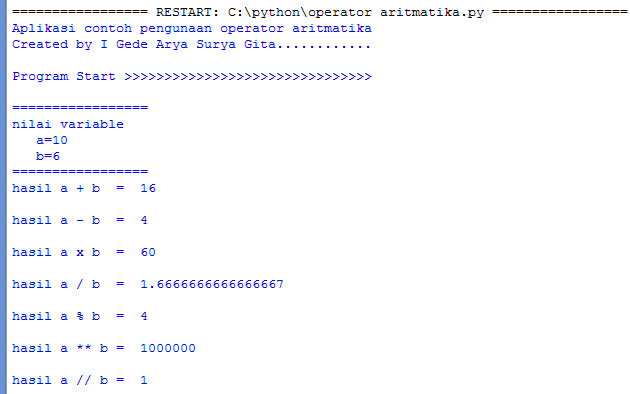
\includegraphics[width=0.25\textwidth]{figures/ctharitmatika}}
 	\caption{Contoh Operator Aritmatika}
 	\label{contoh}
\end{figure}

\vspace{12pt}
\noindent 
Bahasa Python mendukung jenis operator berikut. \par
\vspace{12pt}
\noindent 
\begin{enumerate}
	\item Operator Aritmatika 
	\item Operator Perbandingan (Relasional) 
	\item Operator Penugasan \par
	\item Operator Logis \par
	\item Bitwise Operator \par
	\item Operator keanggotaan \par
	\item Operator Identitas \par
\end{enumerate}


Mari kita lihat semua operator satu per satu. \par
\vspace{12pt}
\noindent 
Operator Aritmatika Python \par
\vspace{12pt}
\noindent 
Asumsikan variabel a memegang 10 dan variabel b memegang 20, maka  \par
\vspace{12pt}
\noindent 
+ Tambahan \par
\noindent 
Menambahkan nilai di kedua sisi operator. \par
\noindent 
Contoh A + b = 30 \par
\vspace{12pt}
\noindent 
- Pengurangan \par
\noindent 
Kurangi operan tangan kanan dari operan tangan kiri. \par
\noindent 
Contoh a - b = -10 \par
\vspace{12pt}
\noindent 
* Perkalian \par
\noindent 
Kalikan nilai di kedua sisi operator \par
\noindent 
Contoh a * b = 200 \par
\vspace{12pt}
\noindent 
/ Divisi \par
\noindent 
Membagi operan tangan kiri dengan tangan kanan operan \par
\noindent 
Contoh B / a = 2 \par
\vspace{12pt}
\noindent 
 $  \%  $ Modulus \par
\noindent 
Membagi operan tangan kiri dengan operan tangan kanan dan mengembalikan sisa \par
\noindent 
Contoh B $  \%  $ a = 0 \par
\vspace{12pt}
\noindent 
** Eksponen \par
\noindent 
Melakukan perhitungan eksponensial (daya) pada operator \par
\noindent 
Contoh A ** b = 10 ke daya 20 \par
\vspace{12pt}
\noindent 
// \par
\vspace{12pt}
\noindent 
Divisi Lantai - Pembagian operan dimana hasilnya adalah hasil bagi di mana angka setelah titik desimal dikeluarkan. $  $Tapi jika salah satu operan negatif, hasilnya berlantai, yaitu terbulatkan dari nol (menuju negatif tak terbatas): \par
\vspace{12pt}
\noindent 
9 // 2 = 4 dan 9.0 // 2.0 = 4.0, -11 // 3 = -4, -11.0 // 3 = -4.0 \par
\vspace{12pt}
\noindent 
Operator Perbandingan Python \par
\vspace{12pt}
\noindent 
Operator ini membandingkan nilai di kedua sisi dan memutuskan hubungan di antara keduanya. $  $Mereka juga disebut operator relasional. \par
\vspace{12pt}
\noindent 
Asumsikan variabel a memegang 10 dan variabel b memegang 20, maka  \par
\vspace{12pt}
\noindent 
== \par
\noindent 
Jika nilai dua operan sama, maka kondisinya menjadi benar. \par
\noindent 
Contoh (a == b) tidak benar \par
\vspace{12pt}
\noindent 
! = \par
\noindent 
Jika nilai dua operan tidak sama, maka kondisinya menjadi benar. \par
\vspace{12pt}
\noindent 
> \par
\noindent 
Jika nilai operan kiri lebih besar dari nilai operan kanan, maka kondisinya menjadi benar. \par
\noindent 
Contoh (a> b) tidak benar \par
\vspace{12pt}
\noindent 
< \par
\noindent 
Jika nilai operan kiri kurang dari nilai operan kanan, maka kondisinya menjadi benar. \par
\noindent 
Contoh (A <b) adalah benar. \par
\vspace{12pt}
\noindent 
> = \par
\noindent 
Jika nilai operan kiri lebih besar dari atau sama dengan nilai operan kanan, maka kondisinya menjadi benar. \par
\noindent 
Contoh (a> = b) tidak benar \par
\vspace{12pt}
\noindent 
<= \par
\noindent 
Jika nilai operan kiri kurang dari atau sama dengan nilai operan kanan, maka kondisinya menjadi benar. \par
\noindent 
Contoh (a <= b) adalah benar. \par
\vspace{12pt}
\noindent 
Operator Penugasan Python \par
\vspace{12pt}
\noindent 
Asumsikan variabel a memegang 10 dan variabel b memegang 20, maka - \par
\vspace{12pt}
\noindent 
= \par
\noindent 
Menetapkan nilai dari operan sisi kanan ke operan sisi kiri \hspace*{4.41in}  \par
\noindent 
Contoh : c = a + b memberi nilai a + b ke c \par
\noindent 
\vspace{12pt}
\noindent 
+ = Tambahkan DAN \par
\noindent 
Ini menambahkan operan kanan ke operan kiri dan menetapkan hasilnya ke operan kiri \par
\noindent 
Contoh : c + = a setara dengan c = c + a \par
\noindent 
\vspace{12pt}
\noindent 
- = Kurangi DAN \par
\noindent 
Ini mengurangi opera kanan dari operan kiri dan menetapkan hasilnya ke operan kiri \par
\noindent 
Contoh : c - = a setara dengan c = c – a \par
\noindent 
\vspace{12pt}
\noindent 
* = Multiply DAN \par
\noindent 
Ini mengalikan operand kanan dengan operan kiri dan menetapkan hasilnya ke operan kiri \par
\noindent 
Contoh : c * = a setara dengan c = c * a \par
\noindent 
\vspace{12pt}
\noindent 
/ = Bagilah dan \par
\noindent 
Ini membagi operan kiri dengan operan kanan dan menetapkan hasilnya ke operan kiri \par
\noindent 
Contoh : C / = a adalah setara dengan c = c / ac / = a adalah setara dengan c = c / a \par
\noindent 
\vspace{12pt}
\noindent 
 $  \%  $ = Modulus DAN \par
\noindent 
Dibutuhkan modulus menggunakan dua operan dan menetapkan hasilnya ke operan kiri \par
\noindent 
Contoh : C $  \%  $ = a setara dengan c = c $  \%  $ a \par
\noindent 
\vspace{12pt}
\noindent 
** = Eksponen DAN \par
\noindent 
Melakukan perhitungan eksponensial (daya) pada operator dan memberikan nilai pada operan kiri \par
\noindent 
Contoh : C ** = a setara dengan c = c ** a \par
\noindent 
\vspace{12pt}
\noindent 
// Divisi Lantai \par
\noindent 
Ini melakukan pembagian lantai pada operator dan memberikan nilai ke operan kiri \par
\noindent 
Contoh : C // = a sama dengan c = c // a \par
\noindent 
\vspace{12pt}
\noindent 
Operator Bitwise Python \par
\vspace{12pt}
\noindent 
Operator Bitwise bekerja pada bit dan melakukan operasi bit by bit. $  $Asumsikan jika a = 60; $  $Dan b = 13; $  $Sekarang dalam format biner mereka akan menjadi seperti berikut - \par

\begin{verbatim}
a = 0011 1100
b = 0000 1101
a & b = 0000 1100
A | b = 0011 1101
a ^ b = 0011 0001
~ a = 1100 0011
\end{verbatim}

Ada beberapa operator Bitwise berikut yang didukung oleh bahasa Python \par
\vspace{12pt}
\noindent 
 $  \&  $ Biner DAN \par
\noindent 
Operator menyalin sedikit ke hasil jika ada di kedua operan \par
\noindent 
Contoh : (A  $  \&  $ b) (berarti 0000 1100) \par
\vspace{12pt}
\noindent 
 $  \vert  $ $  $Biner ATAU \par
\noindent 
Ini salinan sedikit jika ada di salah satu operan. \par
\noindent 
Contoh : (A  $  \vert  $ b) = 61 (berarti 0011 1101) \par
\vspace{12pt}
\noindent 
 $  \string^  $ Biner XOR \par
\noindent 
Ini salinan bit jika diatur dalam satu operand tapi tidak keduanya. \par
\noindent 
Contoh : (A  $  \string^  $ b) = 49 (berarti 0011 0001) \par
\vspace{12pt}
\noindent 
 $  \sim  $ Binary Ones Complement \par
\noindent 
Ini tidak mencolok dan memiliki efek bit 'flipping'. \par
\noindent 
Contoh : ( $  \sim  $ A) = -61 (berarti bentuk pelengkap 1100 0011 dalam 2 karena nomor biner yang ditandatangani \par
\vspace{12pt}
\noindent 
<< Pergeseran Kiri Biner \par
\noindent 
Nilai operan kiri dipindahkan ke kiri oleh jumlah bit yang ditentukan oleh operan kanan. \par
\noindent 
Contoh : Sebuah << = 240 (berarti 1111 0000) \par
\vspace{12pt}
\noindent 
>> Binary Right Shift \par
\noindent 
Nilai operan kiri dipindahkan tepat dengan jumlah bit yang ditentukan oleh operan kanan. \par
\noindent 
Contoh : a >> = 15 (berarti 0000 1111) \par
\vspace{12pt}
\noindent 
Operator Logika Python \par
\vspace{12pt}
\noindent 
Ada beberapa operator logis berikut yang didukung oleh bahasa Python. $  $Asumsikan variabel a memegang 10 dan variabel b memegang 20 kemudian \par
\vspace{12pt}
\noindent 
Digunakan untuk membalik keadaan logis operannya. \par
\vspace{12pt}
\noindent 
Keanggotaan Python Operator \par
\vspace{12pt}
\noindent 
Operator keanggotaan Python menguji keanggotaan secara berurutan, seperti senar, daftar, atau tupel. $  $Ada dua operator keanggotaan seperti yang dijelaskan di bawah ini \par
\vspace{12pt}
\noindent 
Di \par
\noindent 
Mengevaluasi ke true jika menemukan sebuah variabel dalam urutan yang ditentukan dan false sebaliknya. \par
\noindent 
Contoh : X di y, di sini menghasilkan 1 jika x adalah anggota dari urutan y. \par
\vspace{12pt}
\noindent 
tidak masuk \par
\noindent 
Mengevaluasi ke true jika tidak menemukan variabel dalam urutan yang ditentukan dan false sebaliknya. \par
\noindent 
Contoh : X tidak di y, di sini tidak menghasilkan 1 jika x bukan anggota urutan y. \par
\vspace{12pt}
\noindent 
Operator Identitas Python \par
\vspace{12pt}
\noindent 
Operator identitas membandingkan lokasi memori dari dua objek. $  $Ada dua operator Identitas yang dijelaskan di bawah ini: \par
\vspace{12pt}
\noindent 
aku s \par
\noindent 
Mengevaluasi ke true jika variabel di kedua sisi operator menunjuk ke objek yang sama dan salah sebaliknya. \par
\noindent 
Contoh: X adalah y, di sini $  $adalah $  $hasil dalam 1 jika id (x) sama dengan id (y). \par
\vspace{12pt}
\noindent 
Tidak \par
\noindent 
Mengevaluasi false jika variabel di kedua sisi operator menunjuk ke objek yang sama dan benar sebaliknya. \par
\noindent 
Contoh: X bukan y, $  $ini bukan $  $hasil 1 jika id (x) tidak sama dengan id (y). \par
\vspace{12pt}
\noindent 
Operator Python Diutamakan \par
\vspace{12pt}
\noindent 
 berikut mencantumkan semua operator dari preseden tertinggi sampai yang terendah. \par
\vspace{12pt}
\noindent 
** \par
\noindent 
Eksponensiasi (naik ke tampuk kekuasaan) \par
\vspace{12pt}
\noindent 
 $  \sim  $ + - \par
\noindent 
Pelengkap, unary plus dan minus (nama metode untuk dua yang terakhir adalah + @ dan - @) \par
\vspace{12pt}
\noindent 
* / $  \%  $ // \par
\noindent 
Kalikan, bagi, modulo dan pembagian lantai \par
\vspace{12pt}
\noindent 
+ - \par
\noindent 
Penambahan dan pengurangan \par
\vspace{12pt}
\noindent 
>> << \par
\noindent 
Pergeseran bitwise kanan dan kiri \par
\vspace{12pt}
\noindent 
 $  \&  $ \par
\noindent 
Bitwise 'DAN' \par
\vspace{12pt}
\noindent 
 $  \string^  $  $  \vert  $ \par
\noindent 
Bitwise eksklusif `OR 'dan reguler` OR' \par
\vspace{12pt}
\noindent 
<= <>> = \par
\noindent 
Operator perbandingan \par
\vspace{12pt}
\noindent 
<> ==! = \par
\noindent 
Operator kesetaraan \par
\vspace{12pt}
\noindent 
= $  \%  $ = / = // = - = + = * = ** = \par
\noindent 
Operator penugasan \par
\vspace{12pt}
\noindent 
Bukan \par
\noindent 
Operator identitas \par
\vspace{12pt}
\noindent 
Bukan di \par
\noindent 
Operator keanggotaan \par
\vspace{12pt}
\noindent 
Tidak atau dan \par
\noindent 
Operator logika \par
\vspace{12pt}
\noindent 
Peran operator dalam proses perhitungan matematika sangatlah penting. Selain $  $operator Aritmatika, Python juga mendukung $  $operator berkondisi $  $yang berfungsi untuk membandingkan suatu nilai dengan nilai yang lain. Operator-operator yang didukung oleh Python yaitu $  $operator Unari $  $( + dan – ) dan $  $operator Binari $  $( +, -, *, /,  $  \%  $, dan **). Pada ekspresi Aritmatika berikut:\vspace{\baselineskip}
\vspace{\baselineskip}
x = y + z \par
\noindent 
y $  $dan $  $z $  $disebut sebagai operan dari operator $  $+. Tabel di bawah ini menjelaskan tentang berbagai macam operator yang digunakan untuk segala perhitungan di Python. \par
\vspace{12pt}
\noindent 
Jika sebuah ekspresi melibatkan lebih dari satu operator, Python secara otomatis akan memilih operator mana yang akan diutamakan dahulu. Sebagai contoh: \par
\begin{verbatim}
>>> x=7+3*6
>>> x
25
>>> y=100/4*5
>>> y
125

\end{verbatim}
Operator $  $** $  $memiliki urutan tertinggi diantara operator lainnya. Operator $  $* $  $mempunyai urutan lebih tinggi daripada operator $  $+, dan operator $  $/ $  $mempunyai urutan yang sama dengan operator $  $*. Pada ekspresi $  $x = 7 + 3 * 6, bagian $  $3 * 6 $  $akan dieksekusi pertama kali menghasilkan $  $18, yang kemudian ditambahkan dengan $  $7. Sedangkan ekspresi $  $y = 100/4*5, bagian $  $100/4dieksekusi terlebih dahulu karena operator $  $/ $  $berada disebelah kiri dari operator $  $*. \par
\vspace{12pt}
\noindent 
Kita dapat mengubah urutan prioritas dari operator Aritmatika dengan menggunakan kurung-buka-kurung-tutup $  $(). Operator $  $() $  $memiliki urutan tertinggi diantara tiga tipe lainnya. Operator $  $() $  $mempunyai urutan dari kiri ke kanan pada ekspresi di dalamnya. Berikut ini contohnya: \par
\vspace{12pt}
\noindent 
>>> x=(7+3)*6\vspace{\baselineskip}
>>> x\vspace{\baselineskip}
60\vspace{\baselineskip}
>>> y=100/(4*5)\vspace{\baselineskip}
>>> y\vspace{\baselineskip}
5\vspace{\baselineskip}
>>> z=7+(5*(8/2)+(4+6))\vspace{\baselineskip}
>>> z\vspace{\baselineskip}
37 \par
\vspace{12pt}
\noindent 
Operator modulus $  $ $  \%  $ $  $akan memberikan nilai sisa dari pembagian integer. Berikut contoh penggunaan operator modulus: \par
\vspace{12pt}
\noindent 
>>> 7  $  \%  $ 3\vspace{\baselineskip}
1\vspace{\baselineskip}
>>> 0  $  \%  $ 3\vspace{\baselineskip}
0\vspace{\baselineskip}
>>> 1.0  $  \%  $ 3.0\vspace{\baselineskip}
1.0 \par
\vspace{12pt}
\noindent 
Operator eksponensial $  $akan memberikan nilai pangkat dari suatu bilangan. Contoh penggunaan operator eksponensial: \par
\vspace{12pt}
\noindent 
>>> 5**2\vspace{\baselineskip}
25\vspace{\baselineskip}
>>> 5**-2\vspace{\baselineskip}
0.04\vspace{\baselineskip}
>>> -5**2\vspace{\baselineskip}
-25\vspace{\baselineskip}
>>> (-5)**2\vspace{\baselineskip}
25 \par
\vspace{12pt}
\noindent 
Operator Penugasan Python \par
\vspace{12pt}
\noindent 
Asumsikan variabel a memegang 10 dan variabel b memegang 20, maka - \par
\vspace{12pt}
\noindent 
= \par
\noindent 
Menetapkan nilai dari operan sisi kanan ke operan sisi kiri \hspace*{4.41in}  \par
\noindent 
Contoh : c = a + b memberi nilai a + b ke c \par
\noindent 
\vspace{12pt}
\noindent 
+ = Tambahkan DAN \par
\noindent 
Ini menambahkan operan kanan ke operan kiri dan menetapkan hasilnya ke operan kiri \par
\noindent 
Contoh : c + = a setara dengan c = c + a \par
\noindent 
\vspace{12pt}
\noindent 
- = Kurangi DAN \par
\noindent 
Ini mengurangi opera kanan dari operan kiri dan menetapkan hasilnya ke operan kiri \par
\noindent 
Contoh : c - = a setara dengan c = c – a \par
\noindent 
\vspace{12pt}
\noindent 
* = Multiply DAN \par
\noindent 
Ini mengalikan operand kanan dengan operan kiri dan menetapkan hasilnya ke operan kiri \par
\noindent 
Contoh : c * = a setara dengan c = c * a \par
\noindent 
\vspace{12pt}
\noindent 
/ = Bagilah dan \par
\noindent 
Ini membagi operan kiri dengan operan kanan dan menetapkan hasilnya ke operan kiri \par
\noindent 
Contoh : C / = a adalah setara dengan c = c / ac / = a adalah setara dengan c = c / a \par
\noindent 
\vspace{12pt}
\noindent 
 $  \%  $ = Modulus DAN \par
\noindent 
Dibutuhkan modulus menggunakan dua operan dan menetapkan hasilnya ke operan kiri \par
\noindent 
Contoh : C $  \%  $ = a setara dengan c = c $  \%  $ a \par
\noindent 
\vspace{12pt}
\noindent 
** = Eksponen DAN \par
\noindent 
Melakukan perhitungan eksponensial (daya) pada operator dan memberikan nilai pada operan kiri \par
\noindent 
Contoh : C ** = a setara dengan c = c ** a \par
\noindent 
\vspace{12pt}
\noindent 
// Divisi Lantai \par
\noindent 
Ini melakukan pembagian lantai pada operator dan memberikan nilai ke operan kiri \par
\noindent 
Contoh : C // = a sama dengan c = c // a \par
\noindent 
\vspace{12pt}
\noindent 
Operator Bitwise Python \par
\vspace{12pt}
\noindent 
Operator Bitwise bekerja pada bit dan melakukan operasi bit by bit. $  $Asumsikan jika a = 60; $  $Dan b = 13; $  $Sekarang dalam format biner mereka akan menjadi seperti berikut - \par
\vspace{12pt}
\noindent 
a = 0011 1100 \par
\vspace{12pt}
\noindent 
b = 0000 1101 \par
\vspace{12pt}
\vspace{12pt}
\noindent 
a  $  \&  $ b = 0000 1100 \par
\vspace{12pt}
\noindent 
A  $  \vert  $ b = 0011 1101 \par
\vspace{12pt}
\noindent 
a  $  \string^  $ b = 0011 0001 \par
\vspace{12pt}
\noindent 
 $  \sim  $ a = 1100 0011 \par
\vspace{12pt}
\noindent 
Ada beberapa operator Bitwise berikut yang didukung oleh bahasa Python \par
\vspace{12pt}
\noindent 
 $  \&  $ Biner DAN \par
\noindent 
Operator menyalin sedikit ke hasil jika ada di kedua operan \par
\noindent 
Contoh : (A  $  \&  $ b) (berarti 0000 1100) \par
\vspace{12pt}
\noindent 
 $  \vert  $ $  $Biner ATAU \par
\noindent 
Ini salinan sedikit jika ada di salah satu operan. \par
\noindent 
Contoh : (A  $  \vert  $ b) = 61 (berarti 0011 1101) \par
\vspace{12pt}
\noindent 
 $  \string^  $ Biner XOR \par
\noindent 
Ini salinan bit jika diatur dalam satu operand tapi tidak keduanya. \par
\noindent 
Contoh : (A  $  \string^  $ b) = 49 (berarti 0011 0001) \par
\vspace{12pt}
\noindent 
 $  \sim  $ Binary Ones Complement \par
\noindent 
Ini tidak mencolok dan memiliki efek bit 'flipping'. \par
\noindent 
Contoh : ( $  \sim  $ A) = -61 (berarti bentuk pelengkap 1100 0011 dalam 2 karena nomor biner yang ditandatangani \par
\vspace{12pt}
\noindent 
<< Pergeseran Kiri Biner \par
\noindent 
Nilai operan kiri dipindahkan ke kiri oleh jumlah bit yang ditentukan oleh operan kanan. \par
\noindent 
Contoh : Sebuah << = 240 (berarti 1111 0000) \par
\vspace{12pt}
\noindent 
>> Binary Right Shift \par
\noindent 
Nilai operan kiri dipindahkan tepat dengan jumlah bit yang ditentukan oleh operan kanan. \par
\noindent 
Contoh : a >> = 15 (berarti 0000 1111) \par
\vspace{12pt}
\noindent 
Operator Perbandingan Python \par
\vspace{12pt}
\noindent 
Operator ini membandingkan nilai di kedua sisi dan memutuskan hubungan di antara keduanya. $  $Mereka juga disebut operator relasional. \par
\vspace{12pt}
\noindent 
Asumsikan variabel a memegang 10 dan variabel b memegang 20, maka  \par
\vspace{12pt}
\noindent 
== \par
\noindent 
Jika nilai dua operan sama, maka kondisinya menjadi benar. \par
\noindent 
Contoh (a == b) tidak benar \par
\vspace{12pt}
\noindent 
! = \par
\noindent 
Jika nilai dua operan tidak sama, maka kondisinya menjadi benar. \par
\vspace{12pt}
\noindent 
> \par
\noindent 
Jika nilai operan kiri lebih besar dari nilai operan kanan, maka kondisinya menjadi benar. \par
\noindent 
Contoh (a> b) tidak benar \par
\vspace{12pt}
\noindent 
< \par
\noindent 
Jika nilai operan kiri kurang dari nilai operan kanan, maka kondisinya menjadi benar. \par
\noindent 
Contoh (A <b) adalah benar. \par
\vspace{12pt}
\noindent 
> = \par
\noindent 
Jika nilai operan kiri lebih besar dari atau sama dengan nilai operan kanan, maka kondisinya menjadi benar. \par
\noindent 
Contoh (a> = b) tidak benar \par
\vspace{12pt}
\noindent 
<= \par
\noindent 
Jika nilai operan kiri kurang dari atau sama dengan nilai operan kanan, maka kondisinya menjadi benar. \par
\noindent 
Contoh (a <= b) adalah benar. \par
\noindent 
Operator Python Diutamakan \par
\vspace{12pt}
\noindent 
 berikut mencantumkan semua operator dari preseden tertinggi sampai yang terendah. \par
\vspace{12pt}
\noindent 
** \par
\noindent 
Eksponensiasi (naik ke tampuk kekuasaan) \par
\vspace{12pt}
\noindent 
 $  \sim  $ + - \par
\noindent 
Pelengkap, unary plus dan minus (nama metode untuk dua yang terakhir adalah + @ dan - @) \par
\vspace{12pt}
\noindent 
* / $  \%  $ // \par
\noindent 
Kalikan, bagi, modulo dan pembagian lantai \par
\vspace{12pt}
\noindent 
+ - \par
\noindent 
Penambahan dan pengurangan \par
\vspace{12pt}
\noindent 
>> << \par
\noindent 
Pergeseran bitwise kanan dan kiri \par
\vspace{12pt}
\noindent 
 $  \&  $ \par
\noindent 
Bitwise 'DAN' \par
\vspace{12pt}
\noindent 
 $  \string^  $  $  \vert  $ \par
\noindent 
Bitwise eksklusif `OR 'dan reguler` OR' \par
\vspace{12pt}
\noindent 
<= <>> = \par
\noindent 
Operator perbandingan \par
\vspace{12pt}
\noindent 
<> ==! = \par
\noindent 
Operator kesetaraan \par
\vspace{12pt}
\noindent 
= $  \%  $ = / = // = - = + = * = ** = \par
\noindent 
Operator penugasan \par
\vspace{12pt}
\noindent 
Bukan \par
\noindent 
Operator identitas \par
\vspace{12pt}
\noindent 
Bukan di \par
\noindent 
Operator keanggotaan \par
\vspace{12pt}
\noindent 
Tidak atau dan \par
\noindent 
Operator logika \par
\vspace{12pt}
\vspace{12pt}

